%%%%%%%%%%%%%%%%%%%%%%%%%%%%%%%%%%%%%%%%%%%%%%%%%%
%  JASA LaTeX Template File
%  To make articles using JASA.cls, Version 1.1
%  September 14, 2019
%%%%%%%%%%%%%%%%%%%%%%%%%%%%%%%%%%%%%%%%%%%%%%%%%%

%% Step 1:
%% Uncomment the style that you want to use:

%%%%%%% For Preprint
%% For manuscript, 12pt, one column style

\documentclass[preprint]{JASA}

%%%%% Preprint Options %%%%%
%% The track changes option allows you to mark changes
%% and will produce a list of changes, their line number
%% and page number at the end of the article.
%\documentclass[preprint,trackchanges]{JASA}


%% NumberedRefs is used for numbered bibliography and citations.
%% Default is Author-Year style.
%% \documentclass[preprint,NumberedRefs]{JASA}

%%%%%%% For Reprint
%% For appearance of finished article; 2 columns, 10 pt fonts

% \documentclass[reprint]{JASA}

%%%%% Reprint Options %%%%%

%% For testing to see if author has exceeded page length request, use 12pt option
%\documentclass[reprint,12pt]{JASA}


%% NumberedRefs is used for numbered bibliography and citations.
%% Default is Author-Year style.
% \documentclass[reprint,NumberedRefs]{JASA}

%% TurnOnLineNumbers
%% Make lines be numbered in reprint style:
% \documentclass[reprint,TurnOnLineNumbers]{JASA}

\usepackage{natbib}



% tightlist command for lists without linebreak
\providecommand{\tightlist}{%
  \setlength{\itemsep}{0pt}\setlength{\parskip}{0pt}}





\begin{document}
%% the square bracket argument will send term to running head in
%% preprint, or running foot in reprint style.

\title[]{Model-Based Similarity Scores for the Comparison of Cartridge
Case Impressions}

% ie
%\title[JASA/Sample JASA Article]{Sample JASA Article}

%% repeat as needed

\author{Joseph Zemmels}
% ie
%\affiliation{Department1,  University1, City, State ZipCode, Country}
\affiliation{Iowa State University}
%% for corresponding author
\email{jzemmels@iastate.edu}
%% for additional information
\thanks{other info}
\author{Heike Hofmann}
% ie
%\affiliation{Department1,  University1, City, State ZipCode, Country}
\affiliation{Iowa State University}
%% for corresponding author

%% for additional information

\author{Susan VanderPlas}
% ie
%\affiliation{Department1,  University1, City, State ZipCode, Country}
\affiliation{University of Nebraska - Lincoln}
%% for corresponding author

%% for additional information


% ie
% \author{Author Four}
% \email{author.four@university.edu}
% \thanks{Also at Another University, City, State ZipCode, Country.}

%% For preprint only,
%  optional, if you want want this message to appear in upper left corner of title page
\preprint{Zemmels, Hofmann, and VanderPlas, Statistical Analysis and
Data Mining}

%ie
%\preprint{Author, JASA}

% optional, if desired:
%\date{\today}
\date{\today}

\begin{abstract}
% Put your abstract here. Abstracts are limited to 200 words for
% regular articles and 100 words for Letters to the Editor. Please no
% personal pronouns, also please do not use the words ``new'' and/or
% ``novel'' in the abstract. An article usually includes an abstract, a
% concise summary of the work covered at length in the main body of the
% article.
Put your abstract here.
\end{abstract}

%% pacs numbers not used

\maketitle

%  End of title page for Preprint option --------------------------------- %

%% See preprint.tex/.pdf or reprint.tex/.pdf for many examples


%  Body of the article
\defcitealias{council_strengthening_2009}{NRC (2009)}
\defcitealias{pcast2016}{PCAST (2016)}

\hypertarget{introduction}{%
\section{Introduction}\label{introduction}}

A \emph{cartride case} is the part of firearm ammunition that houses the
projectile and propulsive device. When a firearm is discharged and the
projectile travels down the barrel, the cartridge case moves in the
opposite direction and slams against the back wall, the \emph{breech
face}, of the firearm. Markings on the breech face are ``stamped'' into
the surface of the cartridge case leaving so-called \emph{breech face
impressions}.

In a traditional examination, forensic examiners use these impressions
analogous to a fingerprint to determine whether two cartridge cases were
fired from the same firearm. First, two cartridge cases are collected -
perhaps one is from a crime scene and the other is collected from a
suspect's gun. An examiner places the two cartridge cases beneath a
``comparison microscope'' that merges the views of two compound
microscopes into a single split view. The examiner assesses the ``degree
of similarity'' between the markings on the cartridge cases and reaches
either an \emph{identification}, meaning the cartridge cases were fired
from the same firearm, an \emph{elimination}, meaning they were fired
from different firearms, or an \emph{inconclusive}, meaning the evidence
is insufficient to make an identification or elimination
\citep{AFTE1992}.\footnote{The AFTE range of conclusions also permits
  the examiner to decide that the evidence is \emph{unsuitable} for
  examination, which can occur if evidence quality is poor; for example,
  a fragment of a cartridge case is recovered rather than a full
  cartridge case.}

Critics of traditional forensic examinations cite a lack of
``foundational validity'' underlying the procedures used by firearm and
toolmark examiners \citep{council_strengthening_2009, pcast2016}. In
particular, examiners rely largely on their subjective findings rather
than on a well-defined procedure to measure similarity.
\citetalias{pcast2016} pushed for ``developing and testing
image-analysis algorithms'' to objectively measure the similarity
between cartridge cases. Some recently proposed methods focus on
measuring similarity using binary rules \textbf{{[}better way to say
that?{]}} \textbf{{[}CITATIONS{]}}. These methods have the benefit of
being interpretable, although recent work has demonstrated that they can
be highly sensitive to parameter choice \citep{Zemmels2023}.

In this paper, we propose a model-based procedure for measuring the
similarity between two digital scans of cartridge cases. Our procedure
measures similarity using a set of numerical features rather than binary
rules. The result is a continuous score obtained by evaluating a trained
statistical model, which adds nuance to the similarity measure past
concluding that the cartridge cases did or did not originate from the
same firearm.

In the following sections, we first review recently proposed algorithms
to compare firearm evidence. We introduce our similarity scoring
pipeline and share results of applying the pipeline to a data set of
cartridge case scans available at \textbf{{[}data repo citation{]}}. We
discuss how our proposed method builds upon previously proposed methods
to obtain nuanced, informative, and robust similarity measures.

\hypertarget{previous-work}{%
\subsection{Previous Work}\label{previous-work}}

Recent proposals for automatic cartridge case scoring algorithms borrow
from image processing and computer vision techniques. For example,
\citet{vorburger_surface_2007} proposed using the cross-correlation
function (CCF) to compare images or scans of cartridge case surfaces.
The CCF measures the similarity between two matrices for all possible
translations of one matrix against the other. Calculating the CCF while
rotating one of the scans therefore allows for estimation of the optimal
translation and rotation, together referred to as the
\emph{registration}, between the two scans; simply choose the
rotation/translation at which the CCF is maximized.
\citet{hare_automatic_2016} used the CCF, among other features, to
compare scans of bullets. \citet{tai_fully_2018} developed an
open-source cartridge case comparison pipeline that compared cartridge
case images using the CCF.

\citet{song_proposed_2013} noted that two matching cartridge cases often
share similar impressions in specific regions, so calculating the CCF
between two full scans may not highlight their similarities. Instead,
\citet{song_proposed_2013} proposed partitioning one cartridge case scan
into a grid of ``cells'' and calculating the CCF between each cell and
the other scan. If two cartridge cases are truly matching, then the
maximum CCF value between each cell and the other scan, particularly the
cells containing distinguishable breech face impressions, should be
relatively large. Furthermore, the cells should ``agree'' on the
registration at which the CCF is maximized. \citet{song_proposed_2013}
outlined the ``Congruent Matching Cells'' algorithm to determine the
number of cells that agree on a particular registration. A cell is
classified as a Congruent Matching Cell (CMC) if its estimated
registration is within some threshold of the median registration across
all cells and its CCF value is above some threshold. A number of
follow-up papers proposed alterations to the the original CMC method
\citep{tong_improved_2015, chen_convergence_2017}. \citet{cmcR}
introduced an open-source implementation of the CMC method in the
\texttt{cmcR} R package. As an alternative to defining Congruent
Matching Cells, \citet{zhang_convergence_2021} proposed using a
clustering algorithm from \citet{Ester1996} to determine the number of
cells in agreement on a specific registration.

Currently, none of these papers have proposed rigorous procedure for
comparing different cartridge case comparison algorithms. This includes
selecting optimal parameters for a specific algorithm.
\citet{Zemmels2023} proposed an optimization criterion to select
parameters for the CMC algorithm. Analogously,
\citet{hare_automatic_2016} developed a validation procedure to select
parameters for a bullet comparison algorithm. In this work, we introduce
a novel cross-validation procedure to learn and test optimal parameters
for this cartridge case algorithm.

\hypertarget{methods}{%
\section{Methods}\label{methods}}

We now discuss the methods behind the comparison algorithm. We divide
the methods into three stages:

\begin{enumerate}
\def\labelenumi{\arabic{enumi}.}
\item
  \textbf{Pre-processing}: prepare cartridge case scans for comparison
\item
  \textbf{Comparing}: compare two cartridge cases and compute similarity
  features
\item
  \textbf{Scoring}: measure the similarity between the two cartridge
  cases using a trained classifier
\end{enumerate}

The following sections detail each of these stages. Throughout, we treat
``surface matrix'' and ``scan'' synonymously.

After taking a topographical scan of the cartridge case surfaces, we
manually annotate the breech face impression region (shown in red). We
automatically pre-process and compare the scans resulting in a
similarity score, either a binary classification or class probability,
derived from a classifier model. As we pointed out in Chapter 2, prosaic
descriptions like the following are insufficient to reproduce an
algorithm. We refer the reader to
\url{https://github.com/jzemmels/jdssvSubmission/tree/main/supplementary-code}
for the source code used to implement the method and derive the results
presented.

\hypertarget{pre-processing}{%
\subsection{Pre-processing}\label{pre-processing}}

We first use the open-source FiX3P web application
(\url{https://github.com/talenfisher/fix3p}) to manually annotate the
breech face impression region. The FiX3P software includes functionality
to ``paint'' the surface of a cartridge case using a computer cursor and
save the painted regions to a \emph{mask.} A mask is a 2D array of
hexidecimal color values of the same dimension as its associated surface
matrix. When initialized, every element of a mask is a shade of brown
(\#cd7f32) by default. Any elements painted over by the user will be
replaced with the user's selected color value.

We pre-process the raw scans by applying a sequence of functions
available in the R packages \texttt{x3ptools} \citep{x3ptools} and
\texttt{cmcR} \citep{cmcR}. \autoref{fig:preProcessEffect} shows the
effect that each function has on the scan surface values. Gray pixels in
each plot represent missing values in the surface matrix. The
\texttt{x3p\_delete} function removes values in the scan based on the
associated mask. Next, the \texttt{preProcess\_removeTrend} function
subtracts a fitted conditional median plane from the surface values to
``level-out'' any global tilt in the scan. The
\texttt{preProcess\_gaussFilter()} function applies a bandpass Gaussian
filter with wavelength cutoff values 16 and 500 microns to remove
small-scale noise and other large-scale structure, which better
highlights the medium-scale breech face impressions. Finally, the
\texttt{preProcess\_erode()} function applies the morphological
operation of erosion with a circular structuring element of radius 12 on
the edge of the non-missing surface values \citep{Haralick1987}. This
has the effect of shaving off values on the interior and exterior edge
of the surface, which are often extreme ``roll-off'' values that unduly
affect the comparing stage if not removed. The final result is a
cartridge case surface matrix with emphasized breech face impressions.

\begin{figure}[htbp]
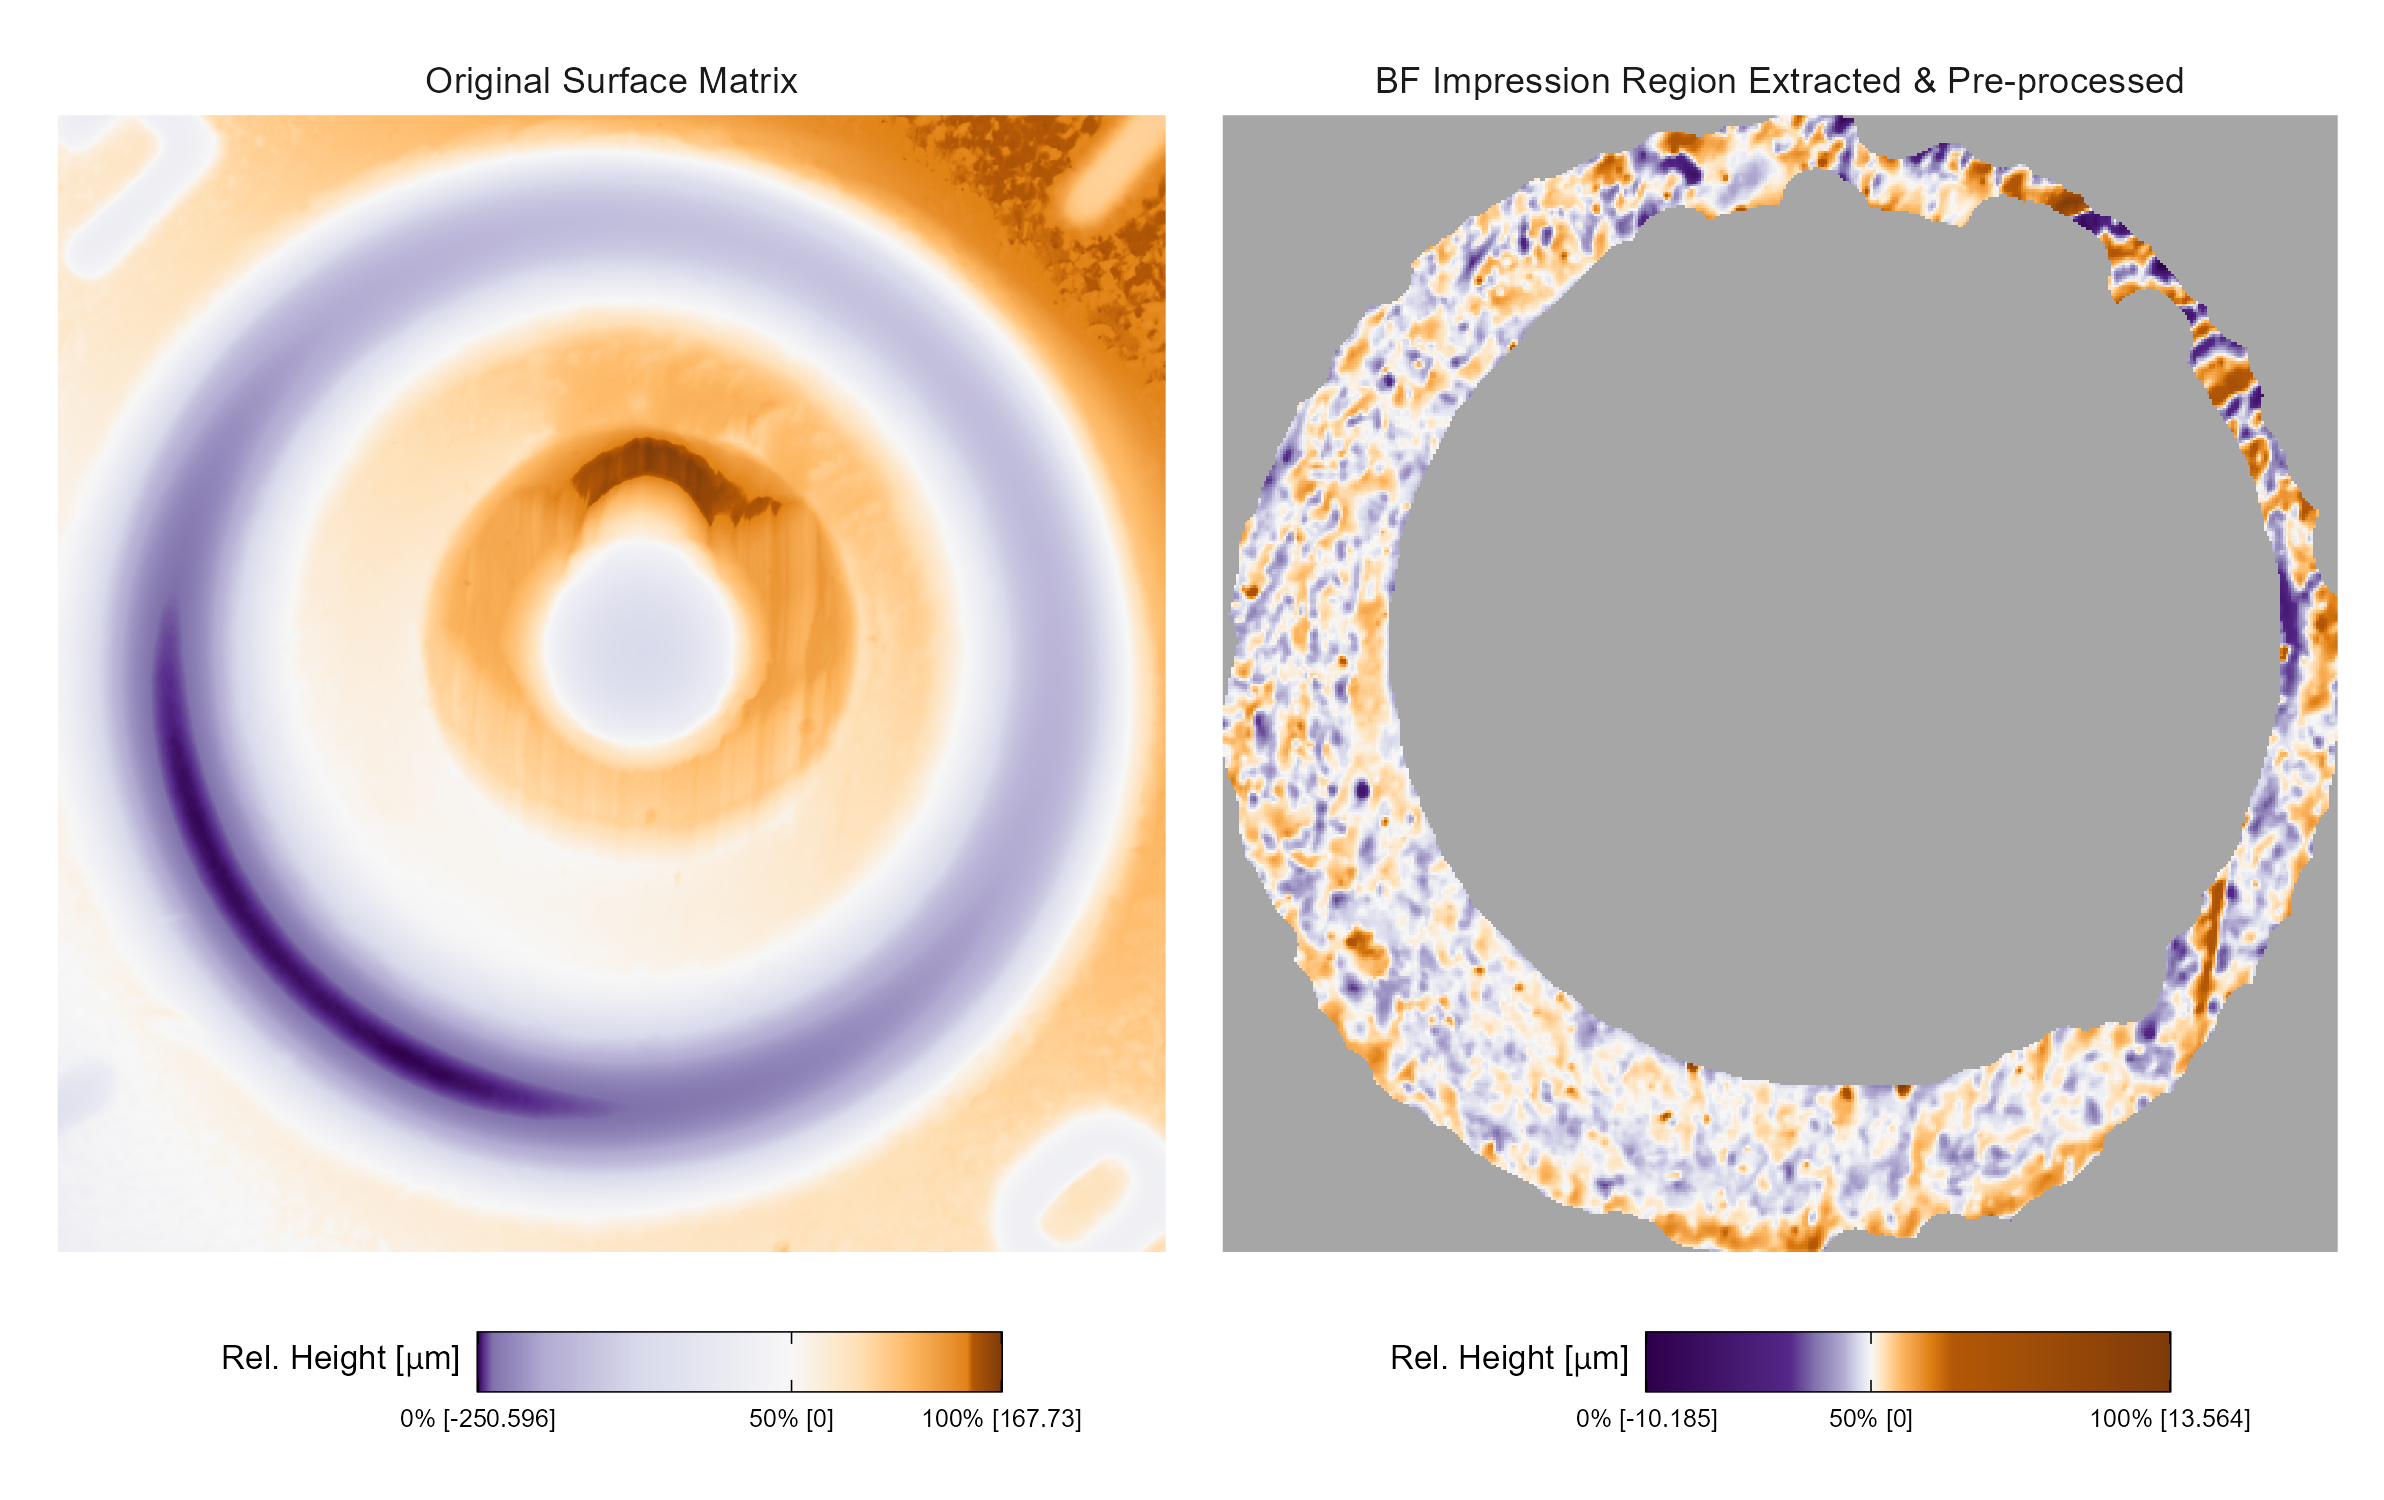
\includegraphics[width=\textwidth]{figures/preProcessEffect} \caption{\label{fig:preProcessEffect} We apply a sequence of pre-processing functions to each scan. Each pre-processing step further emphasizes the breech face impressions in the scan.}\label{fig:unnamed-chunk-3}
\end{figure}

Next, we compute a set of similarity features for two pre-processed
cartridge case scans.

\hypertarget{comparing}{%
\subsection{Comparing}\label{comparing}}

In this section, we introduce a set of similarity features for two
cartridge case scans. We calculate features at two scales: between two
full scans and between individual cells. Analogous to how a forensic
examiner uses a comparison microscope with different magnification
levels, this allows us to assess the similarity between two scans at the
macro and micro levels.

\hypertarget{notational-conventions}{%
\subsubsection{Notational Conventions}\label{notational-conventions}}

First, we introduce notation that will be used to define the features.
Let \(A\) and \(B\) denote two surfaces matrices that we wish to
compare. For simplicity, we assume \(A,B \in \mathbb{R}^{k \times k}\)
for a positive integer
\(k\).\footnote{This assumption of equally-sized, square matrices is easily enforced by padding the matrices with additional missing values.
Due to the presence of (structurally) missing values around the breech face impression region, additional padding does not interfere with the structure of the scan.}
We use lowercase letters and subscripts to denote a particular value of
a matrix: \(a_{ij}\) is the value in the \(i\)-th row and \(j\)-th
column, indexed starting from the top-left corner, of matrix \(A\). In
the following sections, we will use the two known-match cartridge cases
in \autoref{fig:matchPair} as example matrices \(A\) and \(B\).

To accommodate structurally missing values, we adapt standard matrix
algebra by encoding the notion of ``missingness'' into the space of real
values as follows: if an element of either matrix \(A\) or \(B\) is
missing, then any element-wise operation including this element is also
missing. Standard matrix algebra holds for non-missing elements. For
example, the addition operator is defined as: \begin{align*}
A \oplus_{NA} B = (a_{ij} \oplus_{NA} b_{ij})_{1 \leq i,j \leq k} = 
\begin{cases}
a_{ij} + b_{ij} & \text{if both $a_{ij}$ and $b_{ij}$ are numbers} \\
NA &\text{otherwise}
\end{cases}
\end{align*} Other element-wise operations such as \(\ominus_{NA}\) are
defined similarly. For readability, we will use standard operator
notation \(+, -, >, <, I(\cdot), ...\) and assume the extended,
element-wise operations as defined above. Note that this definition of
dealing with missing values is consistent with a setting of
\texttt{na.rm\ =\ FALSE} in terms of calculations in R
\citep{Rlanguage}.

\begin{figure}[htbp]
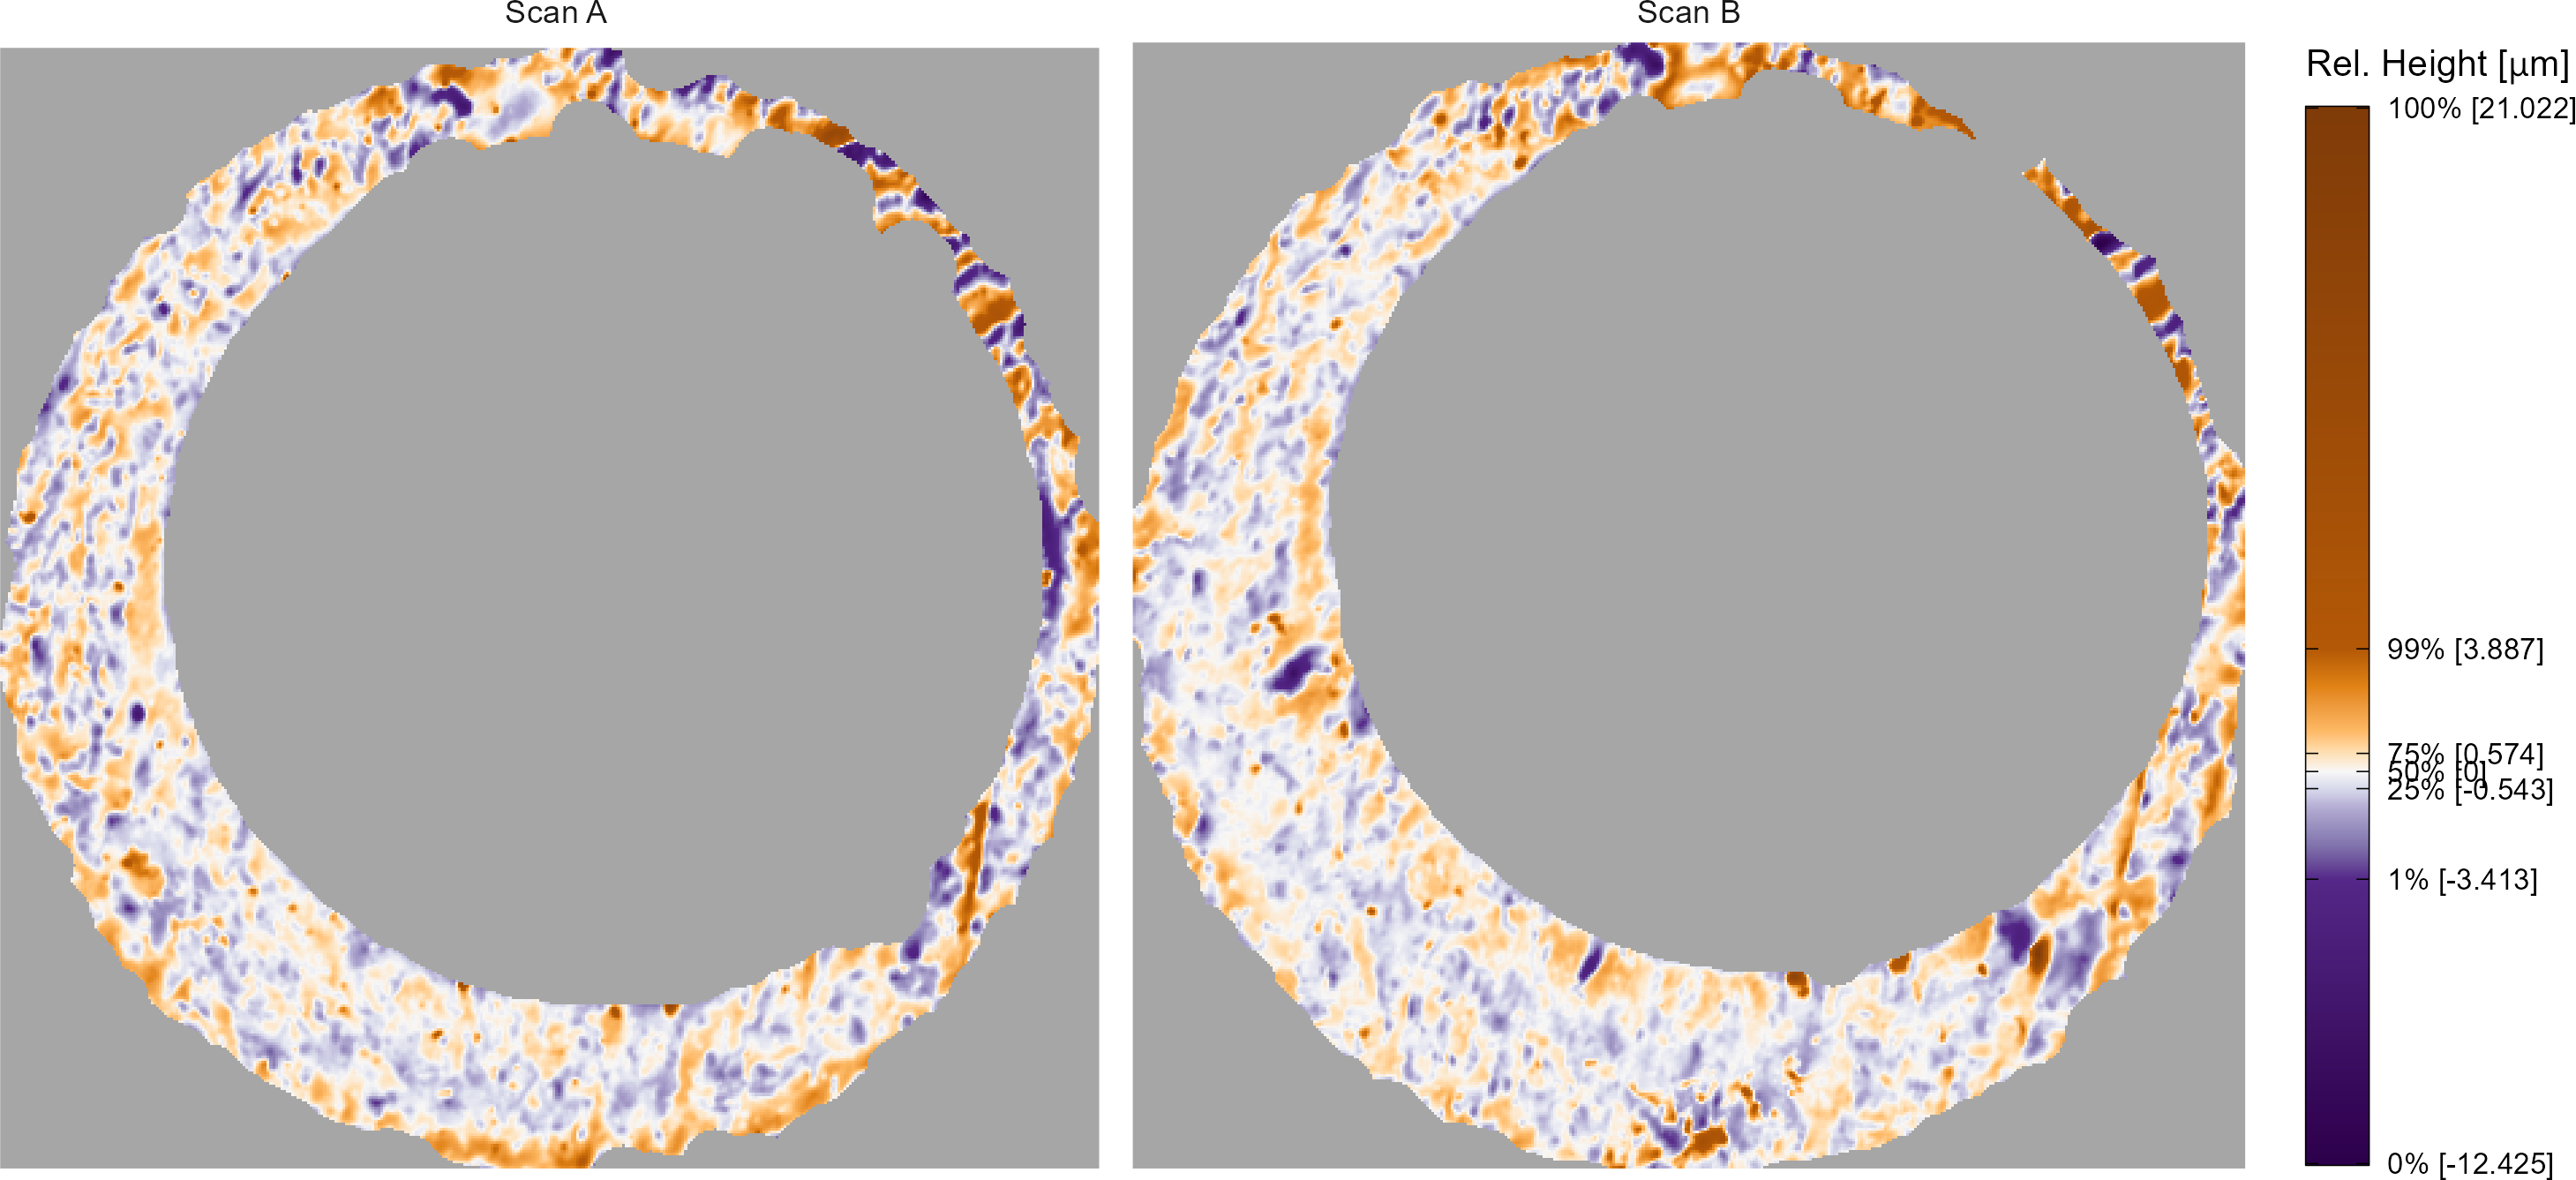
\includegraphics[width=\textwidth]{figures/matchPair} \caption{\label{fig:matchPair} A matching pair of processed cartridge case scans. We measure the similarity between these cartridge cases using the distinguishable breech face impressions on their surfaces.}\label{fig:unnamed-chunk-5}
\end{figure}

\hypertarget{registration-estimation}{%
\subsubsection{Registration Estimation}\label{registration-estimation}}

A critical step in comparing \(A\) and \(B\) is to find a transformation
of \(B\) such that it aligns best to \(A\) (or vice versa). In image
processing, this is called \emph{image registration.} Noting that \(A\)
and \(B\) are essentially grayscale images with structurally missing
values, we rely on a standard image registration technique
\citep{Brown1992}.

In our application, a registration is composed of a discrete translation
by \((m,n) \in \mathbb{Z}^2\) and rotation by
\(\theta \in [-180^\circ,180^\circ]\). To determine the optimal
registration, we calculate the \emph{cross-correlation function} (CCF)
between \(A\) and \(B\), which measures the similarity between \(A\) and
\(B\) for every possible translation of \(B\), denoted \((A \star B)\).
We estimate the registration by calculating the maximum CCF value across
a range of rotations of matrix \(B\). Let \(B_\theta\) denote \(B\)
rotated by an angle \(\theta \in [-180^\circ,180^\circ]\) and
\(b_{\theta_{mn}}\) the \(m,n\)-th element of \(B_\theta\). Then the
estimated registration \((m^*,n^*,\theta^*)\) is:

\[
(m^*,n^*,\theta^*) = \arg \max_{m,n,\theta} (a \star b_\theta)_{mn}.
\]

In practice we consider a discrete grid of rotations
\(\pmb{\Theta} \subset [-180^\circ,180^\circ]\). The registration
procedure is outlined in \autoref{alg:registration}. We refer to the
matrix that is rotated as the ``target.'' The result is the estimated
registration of the target matrix to the ``source'' matrix.

\begin{algorithm}[htbp]
\KwData{Source matrix $A$, target matrix $B$, and rotation grid $\pmb{\Theta}$}
\KwResult{Estimated registration of $B$ to $A$, $(m^*,n^*,\theta^*)$, and cross-correlation function maximum, $CCF_{\max}$}
\For{$\theta \in \pmb{\Theta}$}{
Rotate $B$ by $\theta$ to obtain $B_\theta$\;
Calculate $CCF_{\max, \theta} = \max_{m,n} (a \star b_{\theta})_{mn}$\;
Calculate translation $[m^*_\theta,n^*_\theta] = \arg \max_{m,n} (a \star b_{\theta})_{mn}$
}
Calculate overall maximum correlation $CCF_{\max} = \max_{\theta} \{CCF_{\max,\theta} : \theta \in \pmb{\Theta}\}$\;
Calculate rotation $\theta^* = \arg \max_{\theta} \{CCF_{\max,\theta} : \theta \in \pmb{\Theta}\}$\;
\Return{Estimated rotation $\theta^*$, translation $m^* = m^*_{\theta^*}$ and $n^* = n^*_{\theta^*}$, and $CCF_{\max}$}
\caption{Image Registration Procedure}
\label{alg:registration}
\end{algorithm}

To accommodate missing values, we also compute the
\emph{pairwise-complete correlation} using only the complete value
pairs, meaning neither value is missing, between \(A\) and \(B\).

\hypertarget{registration-based-features}{%
\subsubsection{Registration-Based
Features}\label{registration-based-features}}

\hypertarget{full-scan-registration}{%
\paragraph{Full-Scan Registration}\label{full-scan-registration}}

We first estimate the registration between two full scans \(A\) and
\(B\) using \autoref{alg:registration} with a rotation grid
\(\pmb{\Theta} = \{-30^\circ, -27^\circ,...,27^\circ,30^\circ\}\). This
results in an estimated registration \((m^*,n^*,\theta^*)\) and
similarity measure \(CCF_{\max}\). We also perform
\autoref{alg:registration} with the roles of \(A\) and \(B\) reversed,
meaning the target scan \(A\) is aligned to source scan \(B\).

To accommodate these two comparison directions, we introduce a new
subscript \(d = A,B\), referring to the source scan in Image
Registration Algorithm. Consequently, we obtain two sets of estimated
registrations, \((m^*_d,n^*_d,\theta^*_d)\) and \(CCF_{\max,d}\), for
\(d=A,B\).\footnote{In reality, the true aligning registrations in the two comparison directions are opposites of each other. However, because we compare discretely-indexed arrays using a nearest-neighbor interpolation scheme, the estimated registrations may differ slightly.}
For \(d = A\), we then apply the registration transformation
\((m^*_A,n^*_A,\theta^*_A)\) to \(B\) to obtain \(B^*\) and compute the
pairwise-complete correlation, \(cor_{\text{full},A}\), between \(A\)
and \(B^*\). We repeat this in the other comparison direction to obtain
\(cor_{\text{full},B}\) and average the two:

\[
cor_{\text{full}} = \frac{1}{2}\left(cor_{A,\text{full}} + cor_{B,\text{full}}\right).
\]

We assume that the \textbf{full-scan pairwise-complete correlation} is
large for truly matching cartridge cases.

\hypertarget{cell-based-registration}{%
\paragraph{Cell-Based Registration}\label{cell-based-registration}}

We next perform a cell-based comparison procedure, which begins with
selecting one of the matrices, say \(A\), as the ``source'' matrix that
is partitioned into a grid of cells. The left side of
\autoref{fig:cellGridExample} shows an example of such a cell grid
overlaid on a scan. Each of these source cells will be compared to the
``target'' matrix, in this case \(B^*\). Because \(A\) and \(B^*\) are
already partially aligned from the full-scan registration procedure, we
compare each source cell to \(B^*\) using a new rotation grid of
\(\pmb{\Theta}'_A = \{\theta^*_A - 2^\circ, \theta^*_A - 1^\circ,\theta^*_A,\theta^*_A + 1^\circ,\theta^*_A + 2^\circ\}\).

We now extend the surface matrix notation introduced previously to
accommodate cells. Let \(A_{t}\) denote the \(t\)-th cell of matrix
\(A\), \(t = 1,...,T_A\) where \(T_A\) is the total number of cells
containing non-missing values in scan \(A\) (e.g., \(T_A = 43\) in
\autoref{fig:cellGridExample}) and let \((a_t)_{ij}\) denote the
\(i,j\)-th element of \(A_t\).

The cell-based comparison procedure is outlined in
\autoref{alg:cellComparison}.

\begin{algorithm}[H]
\KwData{Source matrix $A$, target matrix $B^*$, grid size $R \times C$, and rotation grid $\pmb{\Theta}'_A$}
\KwResult{Estimated translations and $CCF_{\max}$ values per cell, per rotation}
Partition $A$ into a grid of $R \times C$ cells\;
Discard cells containing only missing values, leaving $T_A$ remaining cells\;
\For{$\theta \in \pmb{\Theta}'_A$}{
Rotate $B^*$ by $\theta$ to obtain $B^*_\theta$\;
\For{$t = 1,...,T_A$}{
Calculate $CCF_{\max, A,t,\theta} = \max_{m,n} (a_t \star b^*_\theta)_{mn}$\;
Calculate translation $[m^*_{A,t,\theta},n^*_{A,t,\theta}] = \arg \max_{m,n} (a_t \star b^*_\theta)_{mn}$
}
}
\Return{$\pmb{F}_A = \{(m^*_{A,t,\theta},n^*_{A,t,\theta}, CCF_{\max,A,t,\theta}, \theta) : \theta \in \pmb{\Theta}'_A, t = 1,...,T_A\}$}
\caption{Cell-Based Comparison Procedure}
\label{alg:cellComparison}
\end{algorithm}

Rather than exclusively returning the registration that maximizes the
overall CCF as in \autoref{alg:registration},
\autoref{alg:cellComparison} returns the set \(\pmb{F}_A\) of
translations and CCF values for each of the \(T_A\) cells and each
rotation in \(\pmb{\Theta}'_A\).

\begin{figure}[htbp]
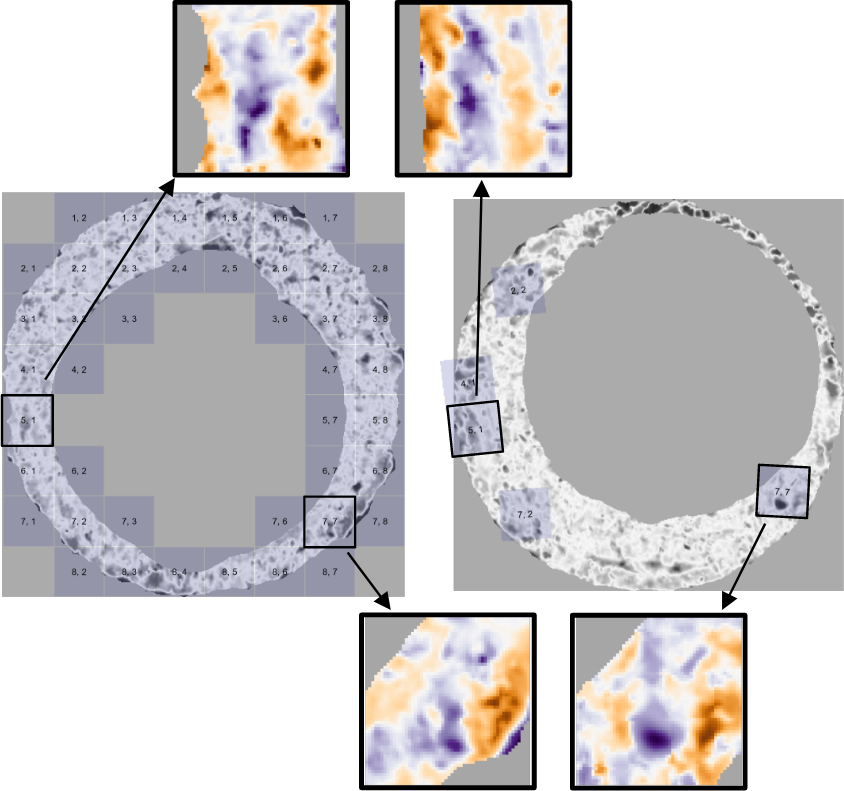
\includegraphics[width=\textwidth]{images/cellGridExample_nonMatch} \caption{\label{fig:cellGridExample} Estimated registrations of cells from a non-match pair of cartridge cases. A source scan (left) is separated into an $8 \times 8$ grid of cells. We exclude cells containing only missing values (visualized here as gray pixels). Each source cell is compared to a target scan (right) to estimate where it aligns best. We show a handful of cells at their estimated alignment in the target scan and magnify the surfaces captured by cell pairs 5, 1 and 7, 7. Although the cartridge case pair is non-matching, we note that there are similarities in the surface markings for these cell pairs.}\label{fig:unnamed-chunk-6}
\end{figure}

\autoref{fig:cellGridExample} shows the estimated registrations of cells
between two non-match cartridge cases. We magnify the surface values
captured by cell pairs 5, 1 and 7, 7 and note the similarities in the
surface values; for example, the dark purple region in the middle of the
cell 7, 7 pair.

Just as with the whole-scan registration, we calculate the
pairwise-complete correlation between each cell \(A_t\) and a matrix
\(B_{\theta,t}^*\) of the same size extracted from \(B^*_{\theta}\)
after translating by \([m^*_{A,\theta},n^*_{A,\theta}]\). From this we
obtain a set of pairwise-complete correlations for each cell and
rotation:
\(\{cor_{A,t,\theta} : t = 1,...,T_A, \theta \in \pmb{\Theta}'_A\}\).

We repeat \autoref{alg:cellComparison} and the pairwise-complete
correlation calculation using \(B\) as the source scan and \(A^*\) as
the target, resulting in cell-based registration set \(\pmb{F}_B\) and
pairwise-complete correlations
\(\{cor_{B,t,\theta} : t = 1,...,T_B, \theta \in \pmb{\Theta}'_B\}\).

For \(d = A,B\) and \(t = 1,...,T_d\), define the cell-wise maximum
pairwise-complete correlation as:

\[
cor_{d,t} = \max_{\theta} \{cor_{d,t,\theta} : \theta \in \pmb{\Theta}'_d\}.
\]

We compute two features, the \textbf{average} and \textbf{standard
deviation of the cell-based pairwise-complete correlations}, using the
correlation data:

\begin{align*}
\overline{cor}_{\text{cell}} &= \frac{1}{T_A + T_B} \sum_{d \in \{A,B\}} \sum_{t=1}^{T_d} cor_{d,t} \\
s_{cor} &= \sqrt{\frac{1}{T_A + T_B - 1} \sum_{d \in \{A,B\}} \sum_{t=1}^{T_d} (cor_{d,t} - \overline{cor}_{\text{cell}})^2}.
\end{align*}

We expect \(\overline{cor}_{\text{cell}}\) and \(s_{cor}\) to be large
for truly matching cartridge case pairs relative to non-matching pairs.

For \(d = A,B\) and \(t = 1,...,T_d\), define the per-cell estimated
translations and rotation as:

\begin{align*}
\theta^*_{d,t} &= \arg \max_{\theta} \{CCF_{\max,d,t,\theta} : \theta \in \pmb{\Theta}'_d\} \\
m^*_{d,t} &= m^*_{\theta^*_{d,t},d,t} \\
n^*_{d,t} &= n^*_{\theta^*_{d,t},d,t}.
\end{align*}

We compute the \textbf{standard deviation of the cell-based estimated
registrations} using the estimated translations and rotations:

\begin{align*}
s_{\theta^*} =  \sqrt{\frac{1}{T_A + T_B - 1} \sum_{d \in \{A,B\}} \sum_{t=1}^{T_d} (\theta^*_{d,t} - \bar{\theta}^*)^2} \\
s_{m^*} =  \sqrt{\frac{1}{T_A + T_B - 1} \sum_{d \in \{A,B\}} \sum_{t=1}^{T_d} (m^*_{d,t} - \bar{m}^*)^2} \\
s_{n^*} = \sqrt{\frac{1}{T_A + T_B - 1} \sum_{d \in \{A,B\}} \sum_{t=1}^{T_d} (n^*_{d,t} - \bar{n}^*)^2}
\end{align*}

where

\begin{align*}
\bar{m}^* &= \frac{1}{T_A + T_B} \sum_{d \in \{A,B\}}\sum_{t=1}^{T_d} m^*_{d,t} \\
\bar{n}^* &= \frac{1}{T_A + T_B} \sum_{d \in \{A,B\}} \sum_{t=1}^{T_d} n^*_{d,t} \\
\bar{\theta}^* &= \frac{1}{T_A + T_B} \sum_{d \in \{A,B\}} \sum_{t=1}^{T_d} \theta^*_{d,t}.
\end{align*}

We expect \(s_{\theta^*}, s_{m^*},s_{n^*}\) to be small for truly
matching cartridge case pairs relative to non-matching pairs.

From the full-scan and cell-based registration procedures, we obtain six
features summarized in \autoref{tab:registrationFeatures}.

\begin{table}[htbp]
\centering
\begin{tabular}{p{.11\linewidth} p{.7\linewidth}}
$cor_{\text{full}}$ & Full-scan pairwise-complete correlation \\
$\overline{cor}_{\text{cell}}$ & Average cell-based pairwise-complete correlation \\
$s_{cor}$ & Standard deviation of the cell-based pairwise-complete correlations \\
$s_{m^*}$ & Standard deviation of the cell-based vertical translations (in microns) \\
$s_{n^*}$ & Standard deviation of the cell-based horizontal translations (in microns) \\
$s_{\theta^*}$ & Standard deviation of the cell-based rotations (degrees)
\end{tabular}
\caption{Six similarity features based on registering full scans and cells.}
\label{tab:registrationFeatures}
\end{table}

\hypertarget{density-based-features}{%
\subsubsection{Density-Based Features}\label{density-based-features}}

We wish to identify when multiple cells agree on, or cluster around, a
particular registration value. However, pursuant with the notion that
only certain regions of matching cartridge cases contain distinctive
markings, it is unreasonable to assume and empirically rare that
\textbf{all} cells agree on a single registration. In fact, it is common
for many cells to disagree on a registration. For example, the left
scatterplot in \autoref{fig:dbscanScatterplot} shows the per-cell
estimated translations \([m^*_{A,t,\theta}, n^*_{A,t,\theta}]\) when
scan \(A\) is used as source and \(B^*\) as target rotated by
\(\theta = 3^\circ\). The right scatterplot shows the per-cell estimated
translations with the roles of \(A\) and \(B^*\) reversed for
\(\theta = -3^\circ\). We see distinctive clusters, the black points, in
both plots among many noisy, gray points. The task is to isolate the
clusters amongst such noise.

We use the Density-Based Spatial Clustering of Applications with Noise
(DBSCAN) algorithm proposed by \citet{Ester1996} to identify clusters.
Compared to other clustering algorithms such as k-means
\citep{MacQueen1967}, DBSCAN does not require a pre-defined number of
expected clusters. Instead, the algorithm forms clusters if the number
of points within an \(\epsilon > 0\) distance of a point exceeds some
pre-defined threshold, \(minPts > 1\). If a point does not belong to a
cluster, then DBSCAN labels that point as ``noise.'' In
\autoref{fig:dbscanScatterplot}, we use DBSCAN with \(\epsilon = 5\) and
\(minPts = 5\) to identify clusters of size 14 and 13, respectively,
visualized as black points. These cluster sizes suggest that the scans
match. Additionally, the mean cluster centers are approximately
opposites of each other:
\((\hat{m}_A,\hat{n}_A,\hat{\theta}_A) \approx (16.9, -16.7, 3^\circ)\)
when \(A\) is used as source compared to
\((\hat{m}_B,\hat{n}_B,\hat{\theta}_B) \approx (-16.2, 16.8, -3^\circ)\)
when \(B^*\) is used as source. This provides further evidence of a
match.

\begin{figure}[htbp]
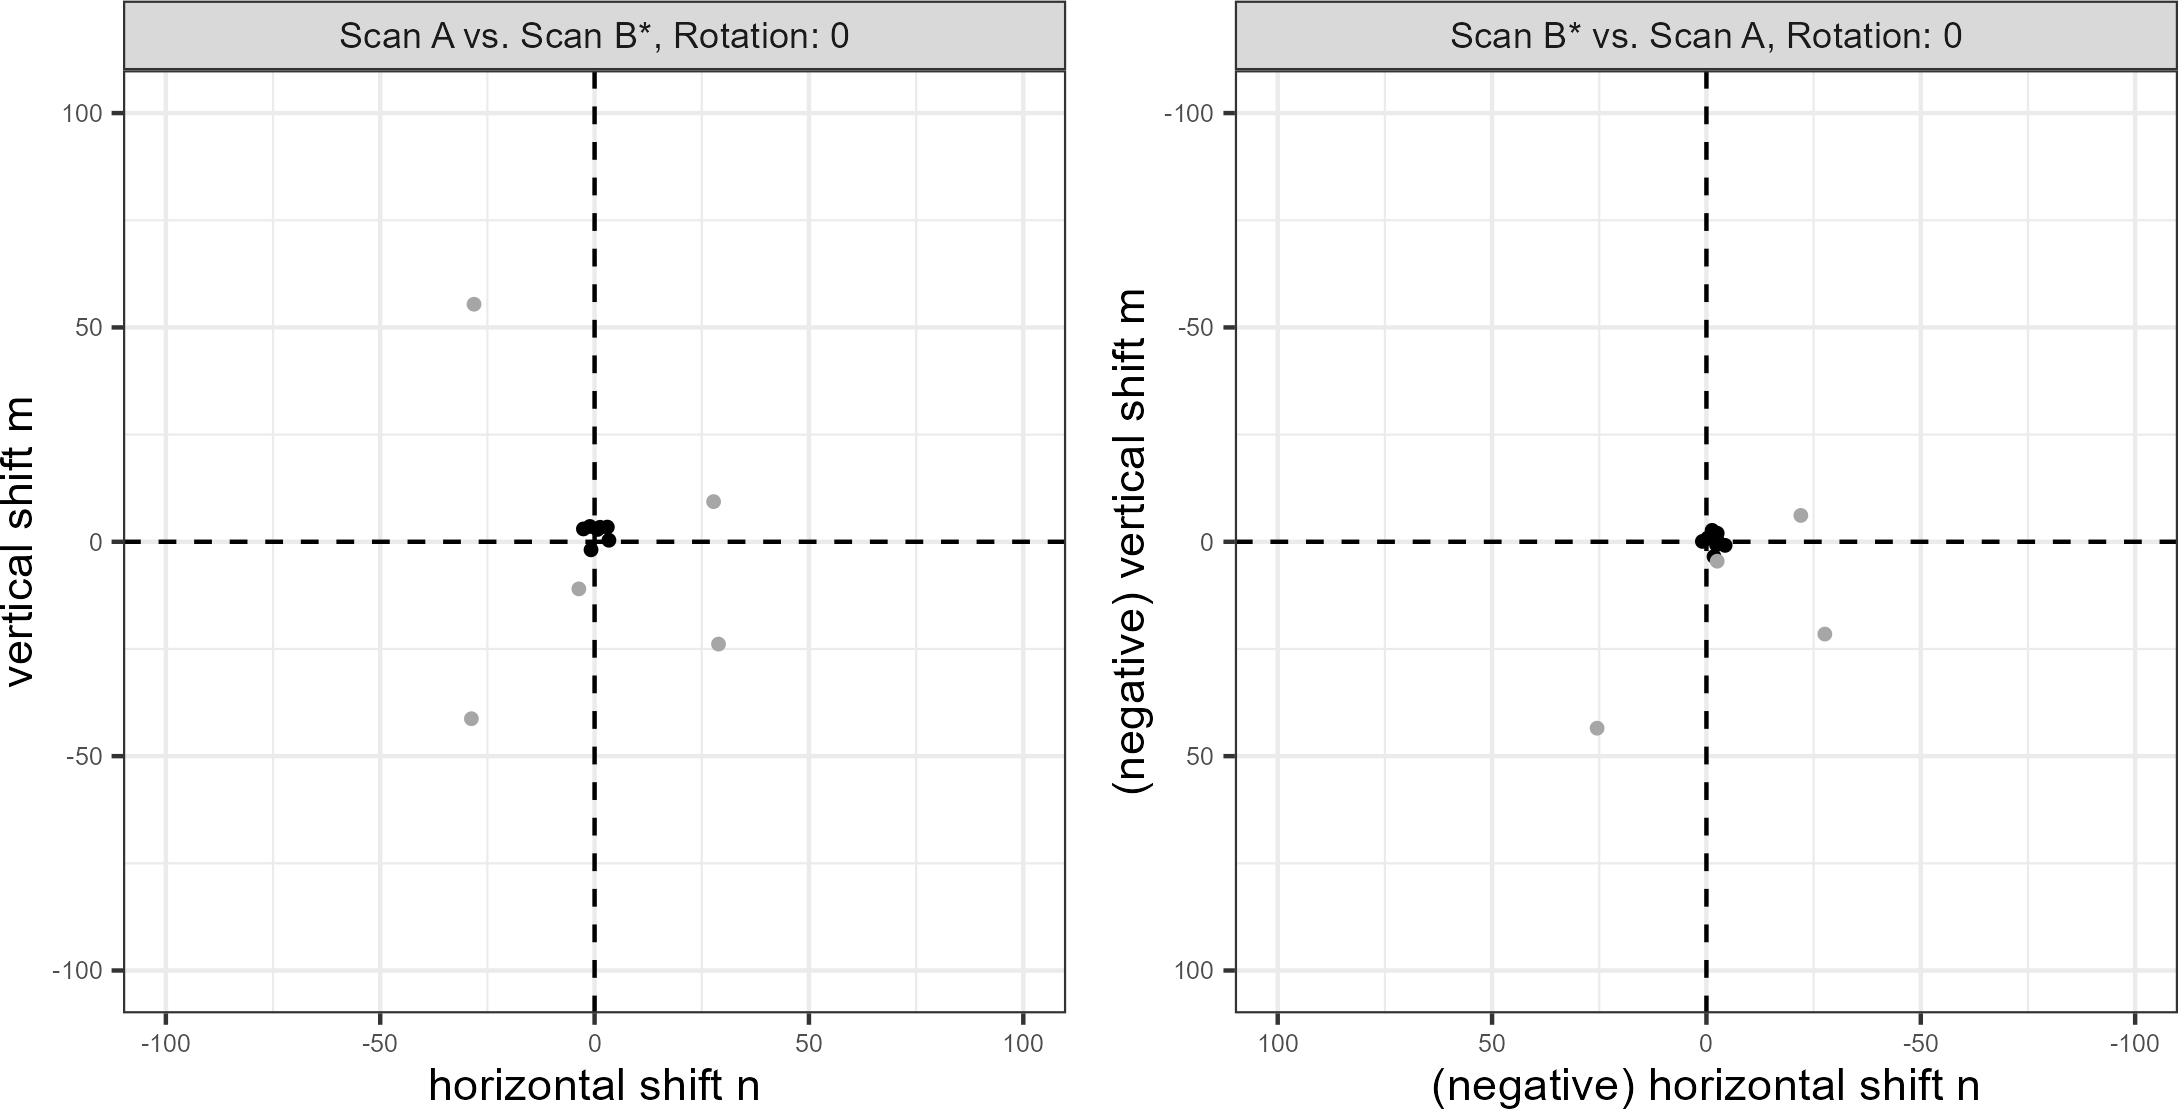
\includegraphics[width=.8\textwidth]{figures/dbscanScatterplot} \caption{\label{fig:dbscanScatterplot} Cluster assignments based on the Density Based Spatial Clustering with Applications to Noise (DBSCAN) algorithm for estimated translations in two comparison directions. Using scan $A$ as source results in a cluster of size 14 (left) compared to 13 when scan $B^*$ is used as source (right). Noting the reversed axes in the right plot, we see that the clusters are located approximately opposite of each other. Points are jittered for visibility.}\label{fig:unnamed-chunk-9}
\end{figure}

To calculate the density-based features, we first use a 2D kernel
density estimator \citep{MASS} to identify the rotation
\(\hat{\theta}_d\) at which the per-cell translations achieve the
highest density. Next, we compute clusters using the DBSCAN algorithm
amongst the estimated translations
\(\{(m^*_{d,t,\hat{\theta}_d},n^*_{d,t,\hat{\theta}_d}) : t = 1,...,T_d\}\)
like those shown in \autoref{fig:dbscanScatterplot}.\footnote{If more
  than one cluster is identified, we binarize the points based on
  whether they were assigned to any cluster or if they are a noise point
  and proceed as if there is only one cluster. We assume that two or
  more clusters form only because of the course rotation grid
  considered. Were a finer grid used, the points would coalesce into a
  single cluster around the true translation value. This assumption has
  empirical support through our experimentation.} Let \(\pmb{C}_d\)
denote the set of cells in the DBSCAN cluster. We treat the mean cluster
centers as the estimated translations \([\hat{m}_d,\hat{n}_d]\).

We calculate four features from the density-based clustering procedure:
\textbf{average DBSCAN cluster size} \(C\), the \textbf{DBSCAN cluster
indicator} \(C_0\), and the \textbf{root sum of squares of the
dens}ity-estimated registrations
\((\Delta_\theta, \Delta_{\text{trans}})\) defined as:

\begin{align*}
C &= \frac{1}{2}\left(|\pmb{C}_A| + |\pmb{C}_B|\right) \\
C_0 &= I(|\pmb{C}_A| > 0 \text{ and } |\pmb{C}_B| > 0)\\
\Delta_\theta &= |\hat{\theta}_A + \hat{\theta}_B| \\
\Delta_{\text{trans}} &= \sqrt{(\hat{m}_A + \hat{m}_B)^2 + (\hat{n}_A + \hat{n}_B)^2}
\end{align*} where \(|\pmb{C}_d|\) denotes the cardinality of
\(\pmb{C}_d\) and \(I(\cdot)\) is the identity function equal to 1 if
the predicate argument ``\(\cdot\)'' evaluates to TRUE and 0 otherwise.
We use both \(C\) and \(C_0\) because of potential missingness in the
values of \(C\) if no cluster is identified. Missing \(C\) values are
imputed using the median non-missing value when fitting classifiers, so
the missingness information is retained in \(C_0\).

For truly matching cartridge case pairs, we expect \(C\) to be large,
\(C_0\) to be 1, and \(\Delta_\theta, \Delta_{\text{trans}}\) to be
small relative to non-matching pairs. We obtain four density-based
features summarized in \autoref{tab:dbscanFeatures}.

\begin{table}[htbp]
\centering
\begin{tabular}{p{.11\linewidth} p{.7\linewidth}}
$C$ & Average DBSCAN cluster size \\
$C_0$ & DBSCAN cluster indicator \\
$\Delta_\theta$ & Absolute sum of the density-estimated rotations (degrees) \\
$\Delta_{\text{trans}}$ & Root sum of squares of the density-estimated translations (in microns)
\end{tabular}
\caption{Four similarity features based on the density-based clustering procedure.}
\label{tab:dbscanFeatures}
\end{table}

\hypertarget{results}{%
\section{Results}\label{results}}

\hypertarget{discussion}{%
\section{Discussion}\label{discussion}}

\hypertarget{conclusion}{%
\section{Conclusion}\label{conclusion}}

\begin{acknowledgments}
This work was partially funded by the Center for Statistics and
Applications in Forensic Evidence (CSAFE) through Cooperative Agreement
70NANB20H019 between NIST and Iowa State University, which includes
activities carried out at Carnegie Mellon University, Duke University,
University of California Irvine, University of Virginia, West Virginia
University, University of Pennsylvania, Swarthmore College and
University of Nebraska, Lincoln.

Additionally, we would like to thank the technicians and staff at the
Roy J. Carver High Resolution Microscopy Facility for collecting the
topographical scans used in this paper.

\end{acknowledgments}

\appendix

% -------------------------------------------------------------------------------------------------------------------
%   Appendix  (optional)

%\appendix
%\section{Appendix title}

%If only one appendix, please use
%\appendix*
%\section{Appendix title}


%=======================================================

%Use \bibliography{<name of your .bib file>}+
%to make your bibliography with BibTeX.

%=======================================================

\bibliography{biblio.bib}


\end{document}
